\documentclass[8pt]{beamer}
\usepackage[utf8]{inputenc}
\usepackage{ulem}
\usepackage{xcolor}
\usepackage{colortbl}
\usepackage{epsfig}
% \usepackage{cancel}
\usepackage{ulem}
% \usepackage{threeparttable} % Joao Pela: 
\usepackage{amsmath}
\usepackage{hyperref}
\usepackage{appendixnumberbeamer}
\usepackage{pdfpages}
% \usepackage{feynmp}         % For latex produced Feynman Diagrams

% Rule for feynmp diagrams to be considered graphics
% \DeclareGraphicsRule{*}{mps}{*}{}
% 
% % New compile sequence for feynmp
% \makeatletter
% \def\endfmffile{%
%   \fmfcmd{\p@rcent\space the end.^^J%
%           end.^^J%
%           endinput;}%
%   \if@fmfio
%     \immediate\closeout\@outfmf
%   \fi
%   \ifnum\pdfshellescape=\@ne
%     \immediate\write18{mpost \thefmffile}%
%   \fi}
% \makeatother

\usetheme{Madrid}

\author[J. Pela]{A. Magnan, P. Dunne,\underline{J. Pela}}
\title{QCD Modelling}
\institute[ICL]{Imperial College London}
\date{2014-05-12}

% The log drawn in the upper right corner.
\logo{\includegraphics[height=0.115\paperheight]{img/Logo_CMSICL.png}}

\begin{document}
\setlength{\unitlength}{1mm}

% ###################################################
\begin{frame}
  \titlepage
\end{frame}

% ###################################################
\begin{frame}{Today's presentation}
 
\begin{block}{Topics}
 
\begin{itemize}
  \item QCD VBF samples definition and motivation.
  \item Definition of a preselection to select real MET QCD.
  \item Analysis strategy.
%   \item Further ideas for the analysis.
\end{itemize}

\end{block}

\end{frame}

% ###################################################
\begin{frame}{QCD VBF sample definition and motivation}

This initial idea was to make a QCD sample with real MET and jets with VBF characteristics.

\begin{block}{Motivations and limitations}
  
\begin{itemize}
  \item The ability to actually make QCD samples with enough statistics to compare with 2012 dataset ($\sim40$ $fb^{-1}$).
  \item Samples with manageable size ($\sim10$ $TB$).
  \item CPU capability able to be produced with Imperial resourced in under 1 month.
  \item RECO filters are prohibitively CPU expensive to be usable. Generator filter are the only feasible option.
\end{itemize}

\end{block}

\vspace{-10px}
\begin{columns}

\column[t]{0.45\linewidth}
\begin{block}{Generator level filters}

\tiny

Generator MET Filter:
\begin{itemize}
  \item $MET_{Generator} = 40.0$ $GeV$ (here the MET is the vectorial sum of all neutrinos $p_{\perp}$)
\end{itemize}

Generator Jets Filter:
\begin{itemize}
  \item Jet selection: 
  \begin{itemize}
    \item \tiny $Jet(p_{\perp})>20$ $GeV$
    \item \tiny $-5.0<Jet(\eta)<5.0$
  \end{itemize}
  \item Dijet selection:
  \begin{itemize}
    \item \tiny $3.2<Dijet(\Delta\eta)<10.0$
    \item \tiny $700<Dijet(m_{jj})<50000$
  \end{itemize}
\end{itemize}

\end{block}

\column[t]{0.45\linewidth}
\begin{block}{Filter efficiencies}
 
\resizebox{\linewidth}{!}{
\begin{tabular}{|l|r|r|r|c|c|c|}
\hline

 & Gen. Ev & Pass MET &	Pass Dijet & MET Filter Eff &	Dijet Filter Eff & Efficiency \\
\hline\hline
QCD-Pt-50to80-pythia6    &	1000000 &	127 &	3&	0,00013&	0,024&	0,000003 \\
QCD-Pt-80to120-pythia6   &	1000000 &	1172&	41&	0,00117&	0,035&	0,000041 \\
QCD-Pt-120to170-pythia6  &	1000000 &	4276&	293&	0,00428&	0,069&	0,000293 \\
QCD-Pt-170to300-pythia6  &	1000000 &	9315&	1012&	0,00932&	0,109&	0,001012 \\
QCD-Pt-300to470-pythia6  &	1000000 &	17956&	2598&	0,01796&	0,145&	0,002598 \\
QCD-Pt-470to600-pythia6  &	1000000 &	23913&	4187&	0,02391&	0,175&	0,004187 \\
\hline
\end{tabular}}

\end{block}

\end{columns}

\end{frame}

% ###################################################
\begin{frame}{Approach to pre-selection definition}

We want to determine a pre-selection that selects mostly real met events in such a way that our QCD VBF + real MET sample together with all MC background samples can describe data (where backgrounds dominated).   

\begin{block}{Baseline selection}
 
\begin{itemize}
  \item Trigger bit selection (include weighting for MC to data matching)
  \item Lepton Veto
  \item Dijet selection (at least 2 jets with):
  \begin{itemize}
    \item $p_{\perp}>50$ $GeV$ 
    \item $|\eta|<4.7$
  \end{itemize}
\end{itemize}

\end{block}

Now we, add cut by cut methodically removing generator bias on distributions in order to reduced QCD fake MET content (not described by MC) to a manageable/negligible level.    

\end{frame}

% ###################################################
\begin{frame}{$\Delta\eta$ cut}

First we need to cut above the turn on the generator dijet $\Delta\eta$ cut in order to remove that bias.

\begin{columns}
 
\column[t]{0.45\linewidth}
\begin{block}{Dijet $\Delta\eta$}
 
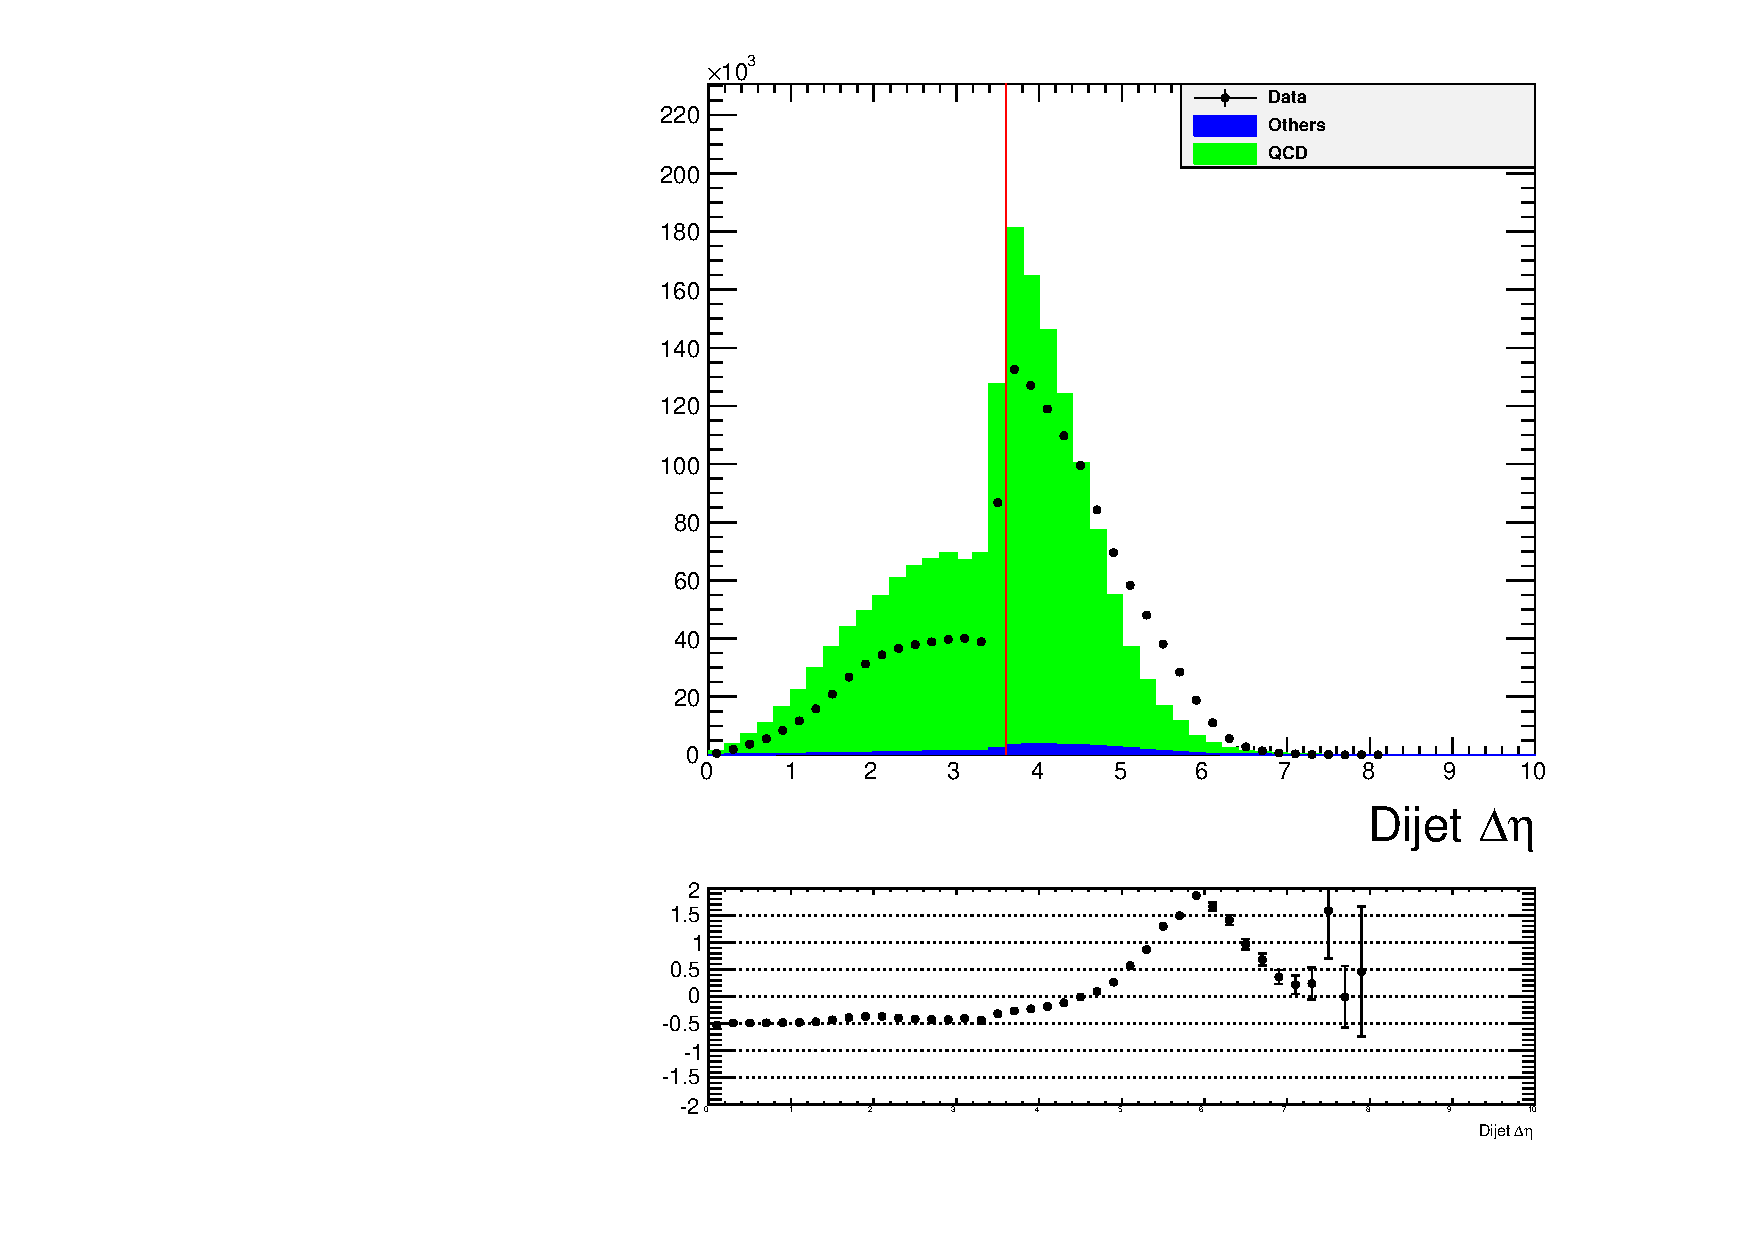
\includegraphics[width=\linewidth]{img/NoCut/dijet_deta.pdf}
 
\end{block}

\column[t]{0.45\linewidth}
\begin{block}{Methodology}

\begin{itemize}
  \item We can see a shape rise around $\Delta\eta\sim3.5$ this is most likely due to the GenJet filter of $\Delta\eta>3.2$
  \item We will cut at $\Delta\eta>3.6$.
  \item We assume that we do not understand distribution on left of the cut so we normalise on the right side:
  \item QCD normalised on $\Delta\eta>3.6$ with $factor = \frac{n_{Data}-n_{\text{other bkg}}}{n_{QCD}}$
  \item Distributions still does not agree in shapes.
\end{itemize}

\end{block}

\end{columns}

\end{frame}

% ###################################################
\begin{frame}{$\Delta\eta$ cut - signal efficiency}
 
\begin{columns}
 
\column[t]{0.45\linewidth}
\begin{block}{Signal Eff. vs $\Delta\eta$}

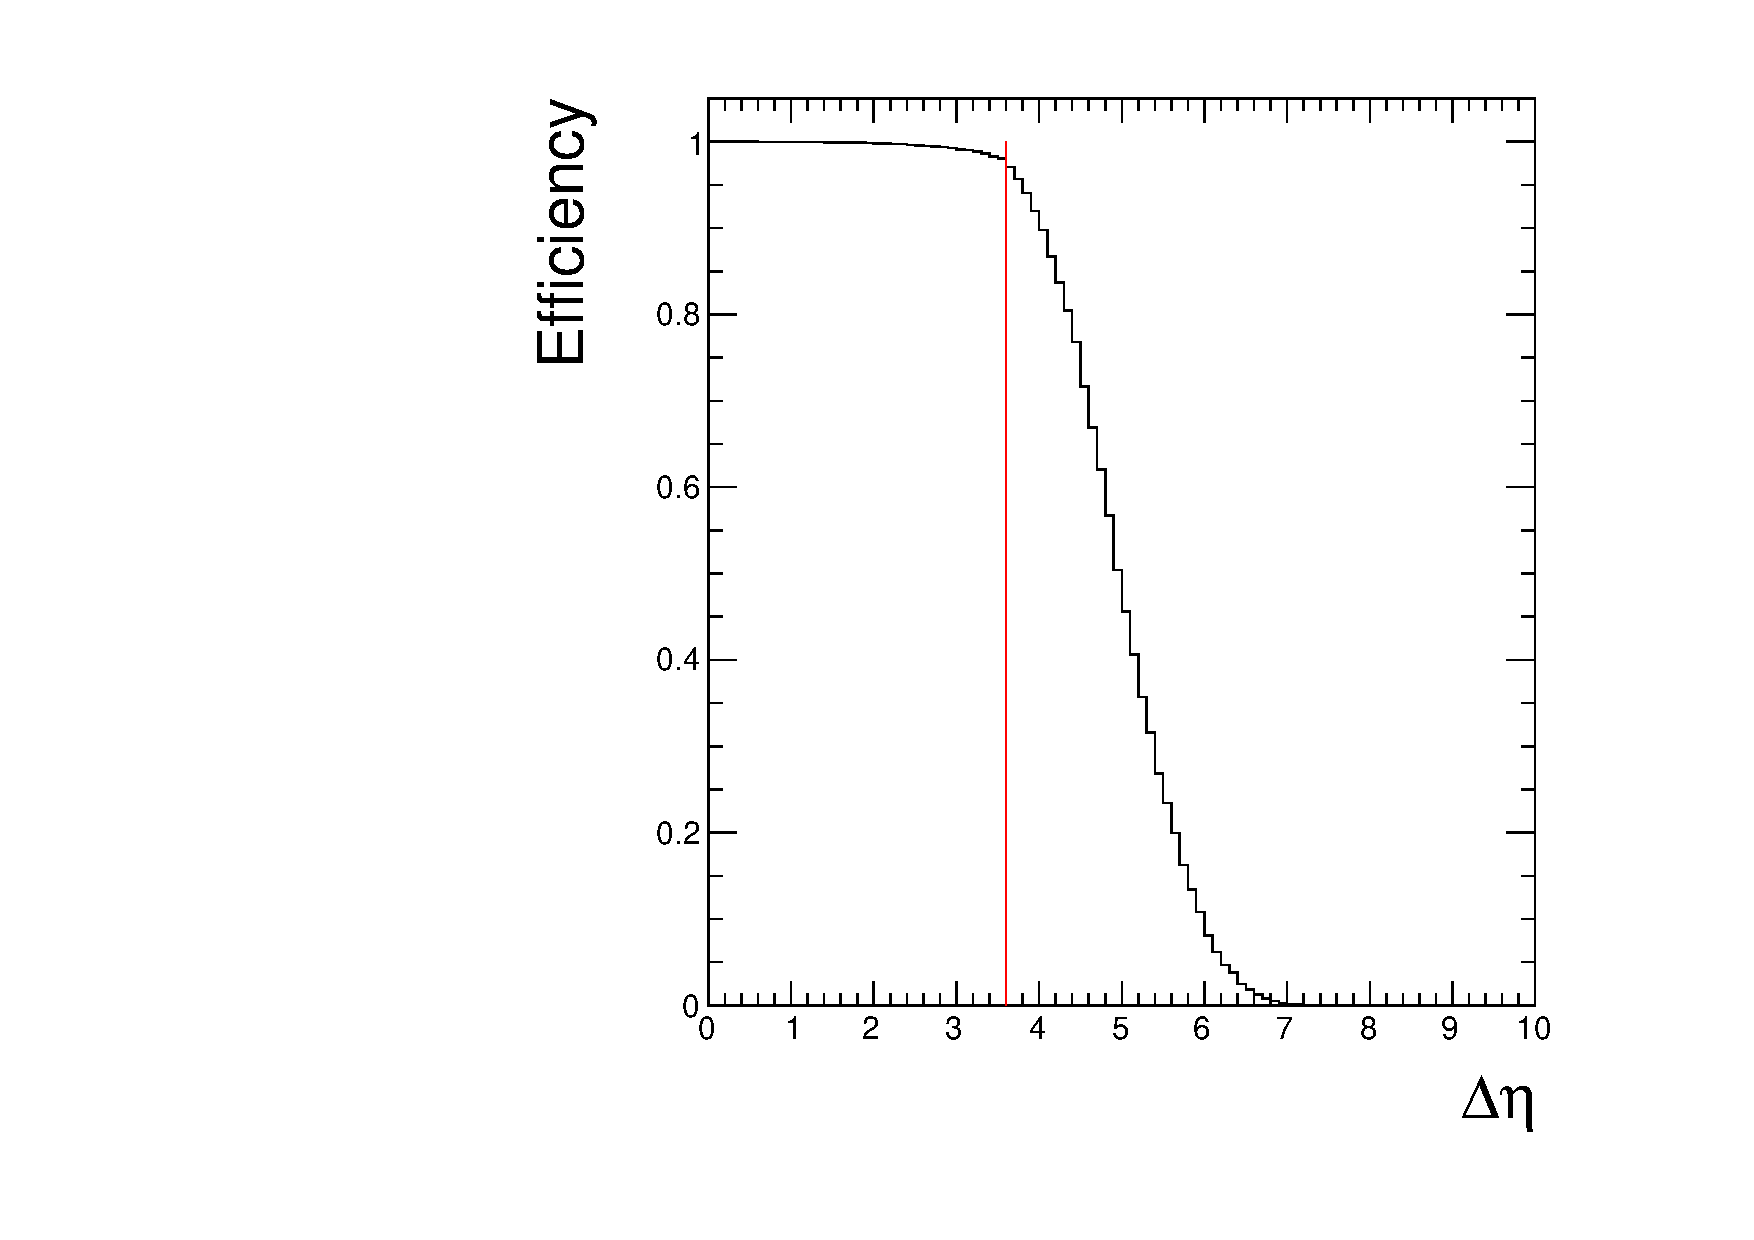
\includegraphics[width=\linewidth]{img/NoCut/DEtaEff.pdf} 

\end{block}

\column[t]{0.45\linewidth}
\begin{block}{Efficiency}

\begin{itemize}
  \item We can now calculate how much is our signal efficiency for $m_{Higgs}=125$ GeV and $BR(Inv)=100\%$ 
  \item Signal Efficiency $\Delta\eta$ (3.6) = $\sim0.97$
  \item Our signal is almost untouched by this cut.
\end{itemize}

\end{block}

\end{columns}

\end{frame}


% ###################################################
\begin{frame}{MET Significance cut}

\begin{columns}
 
\column[t]{0.45\linewidth}
\begin{block}{MET Significance cut}
 
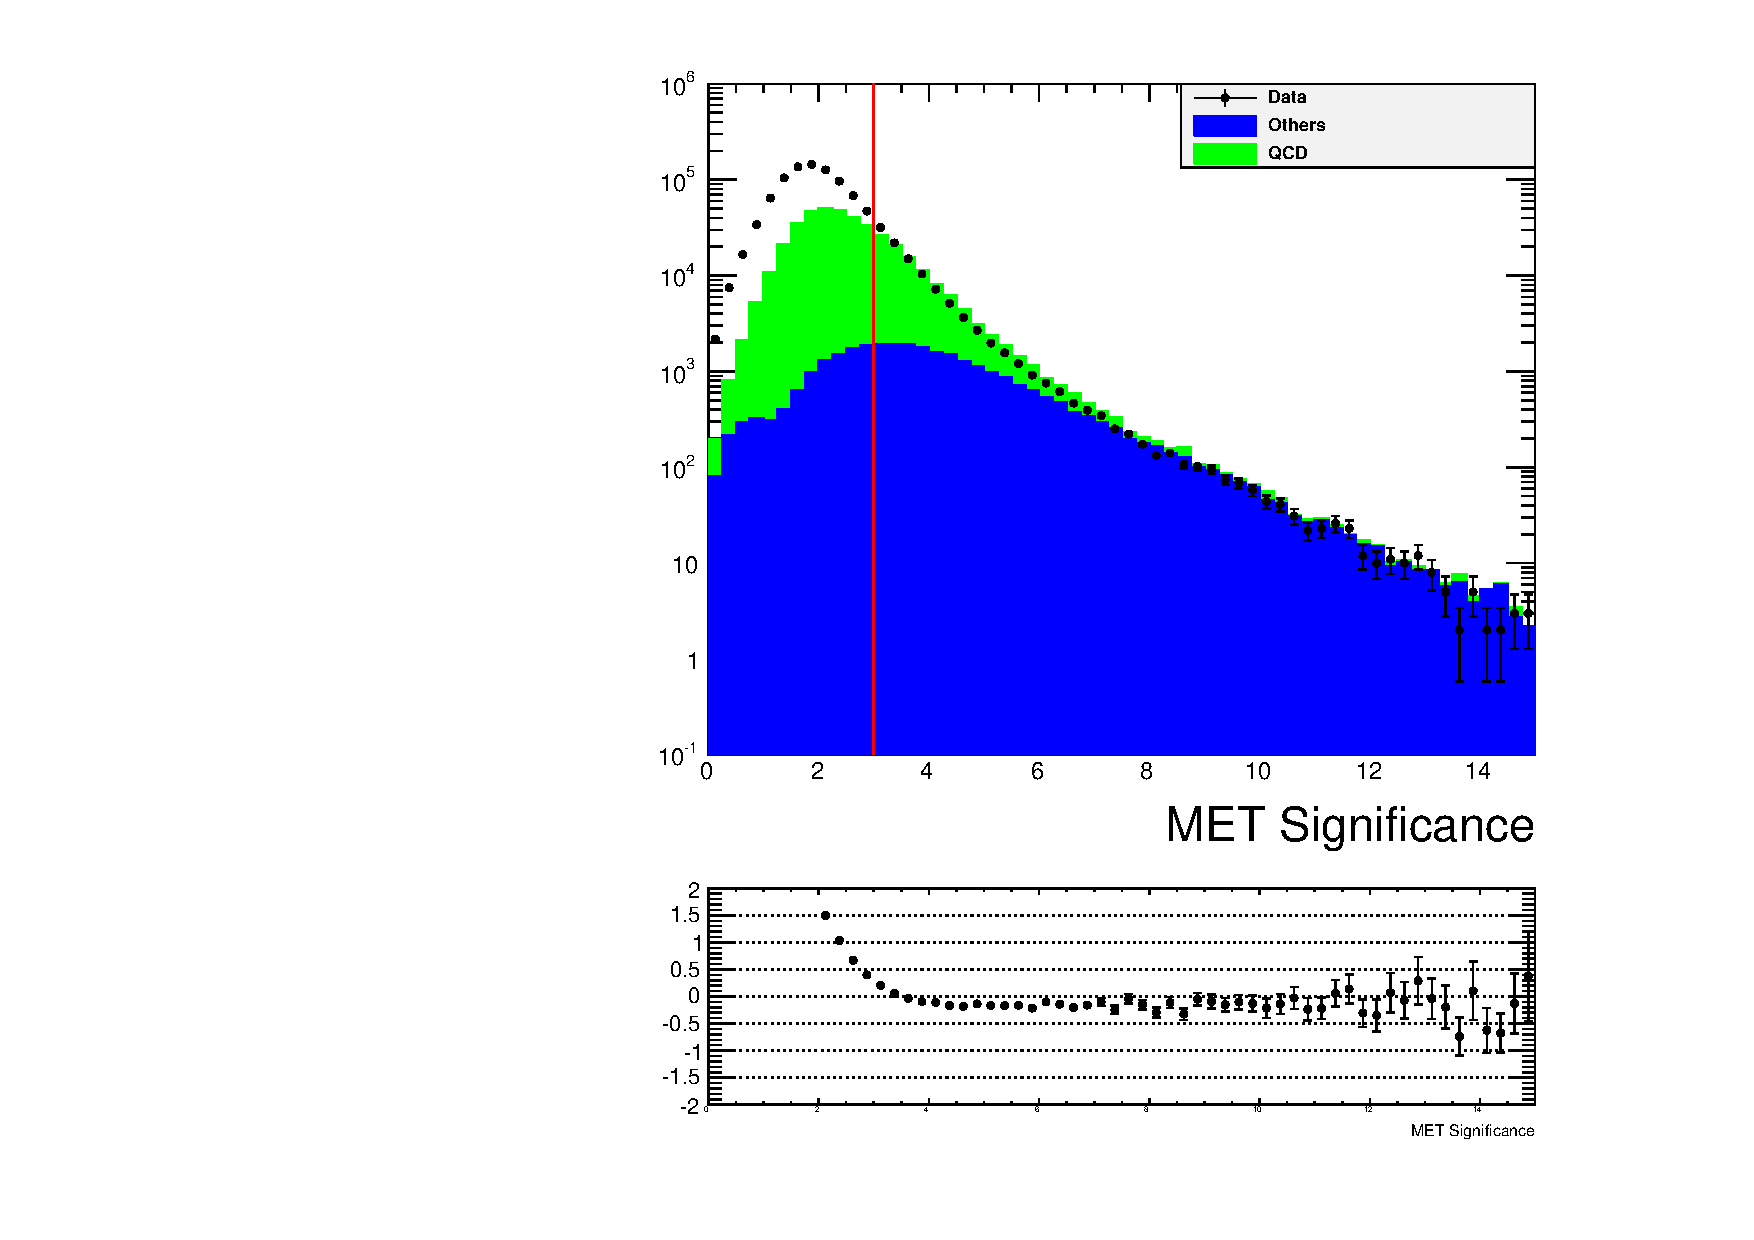
\includegraphics[width=\linewidth]{img/DEta3p6/metSig_LogY.pdf}

\end{block}

\column[t]{0.45\linewidth}
\begin{block}
 
\begin{itemize}
  \item We know that QCD Fake MET events will typically have low MET Significance
  \item We can slide or cut and normalisation window from high to low values and stop when QCD sample does not describe data well anymore due to the raising percentage of QCD fake MET events.
  \item A good value is $MET_{Significance} = 3.0$ (or 3 sigma significance)
  \item QCD normalised on $MET_{Significance}>3.6$ with $factor = \frac{n_{Data}-n_{\text{other bkg}}}{n_{QCD}}$
  \item Above the cut distributions match reasonably.
\end{itemize}

\end{block}

\end{columns}

\end{frame}

% ###################################################
\begin{frame}{MET Significance cut - signal efficiency}
 
\begin{columns}
 
\column[t]{0.45\linewidth}
\begin{block}{Signal Eff. vs MET Significance}

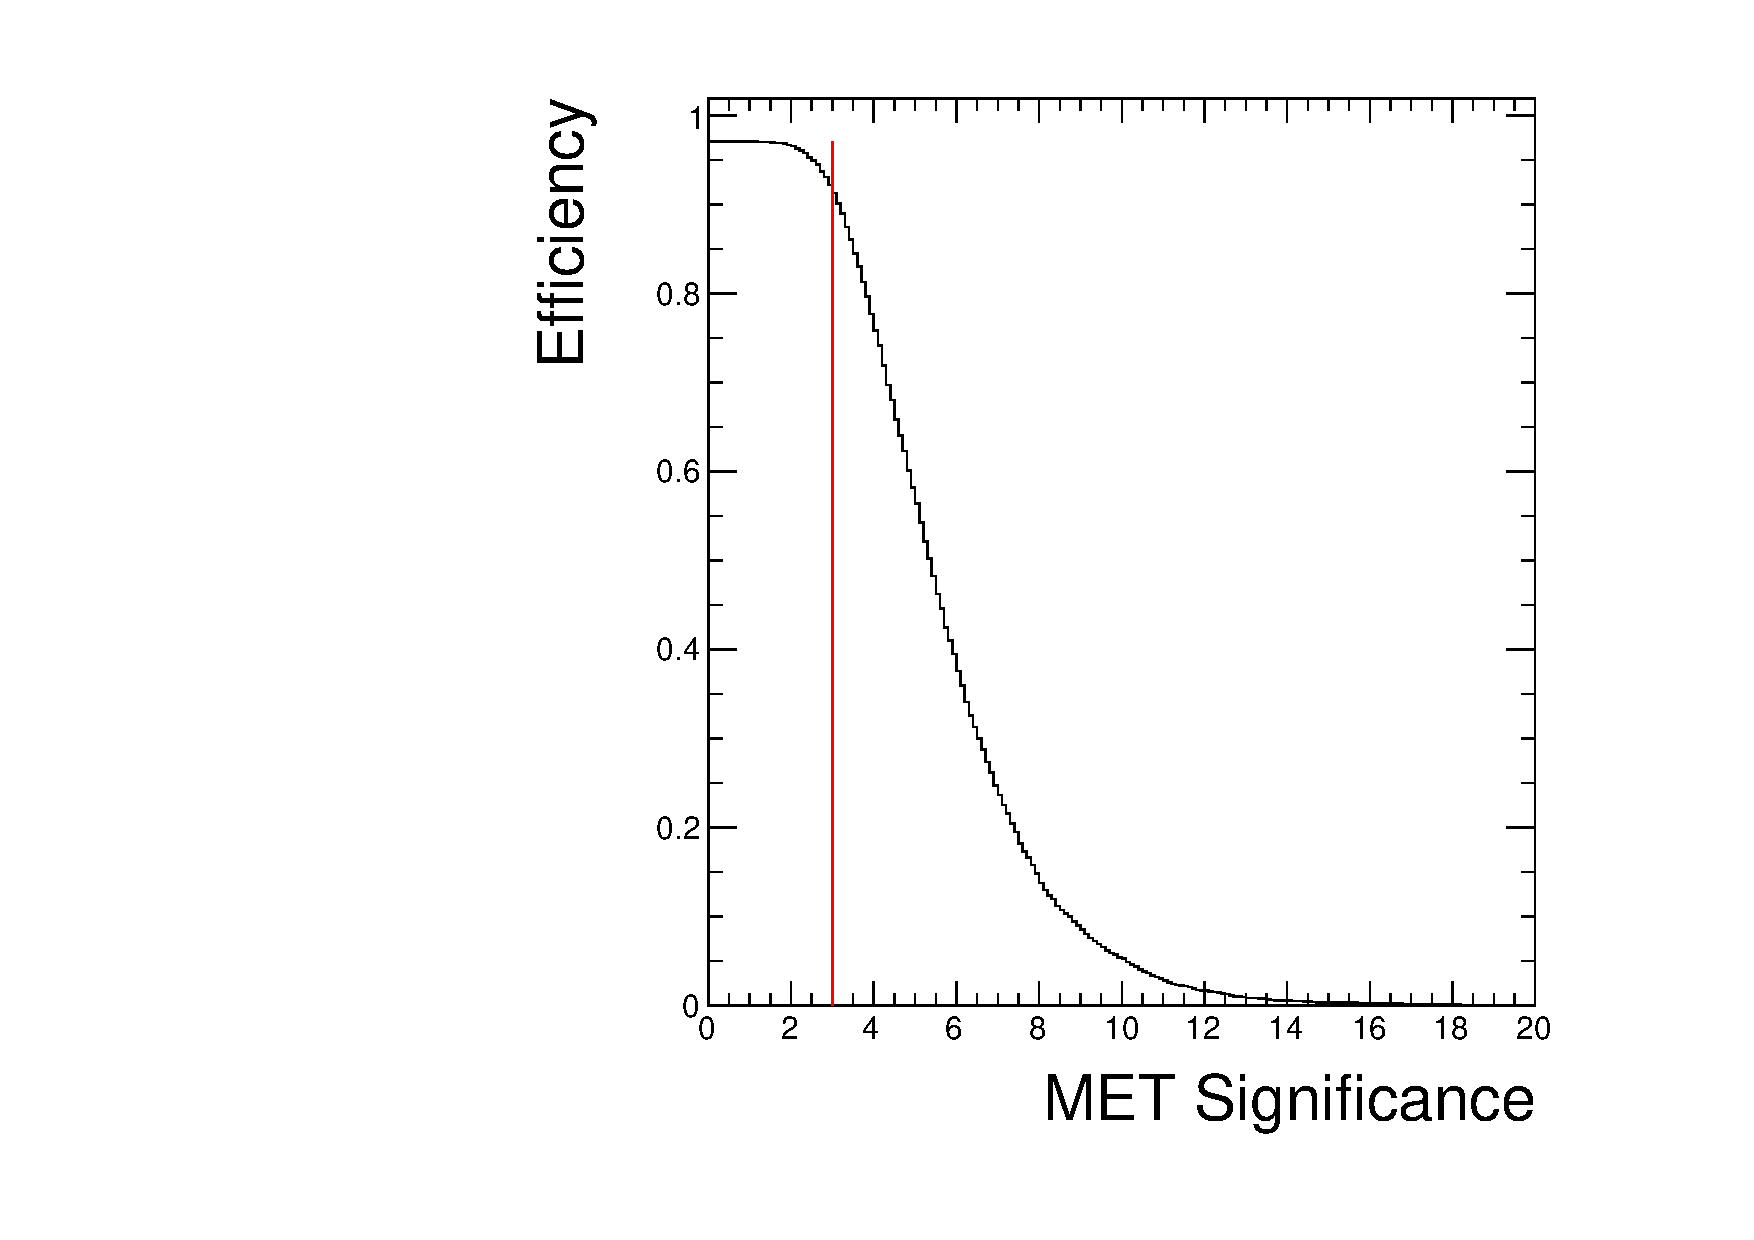
\includegraphics[width=\linewidth]{img/DEta3p6/DEta3p6_metSigEff.pdf} 

\end{block}

\column[t]{0.45\linewidth}
\begin{block}{}

Taking into account the previous cut we can calculate:
\begin{itemize}
  \item Again for signal of $m_{Higgs}=125$ GeV and $BR(Inv)=100\%$ 
  \item Signal Efficiency MET Significance (3.0) = $\sim0.91$
  \item Our signal still remains largely untouched.
\end{itemize}

\end{block}

\end{columns}

\end{frame}


% ###################################################
\begin{frame}{$Min(\Delta\phi(jet_{x},MET))$ cut}

\begin{columns}
 
\column[t]{0.45\linewidth}
\begin{block}{$Min(\Delta\phi(jet_{x},MET))$}
 
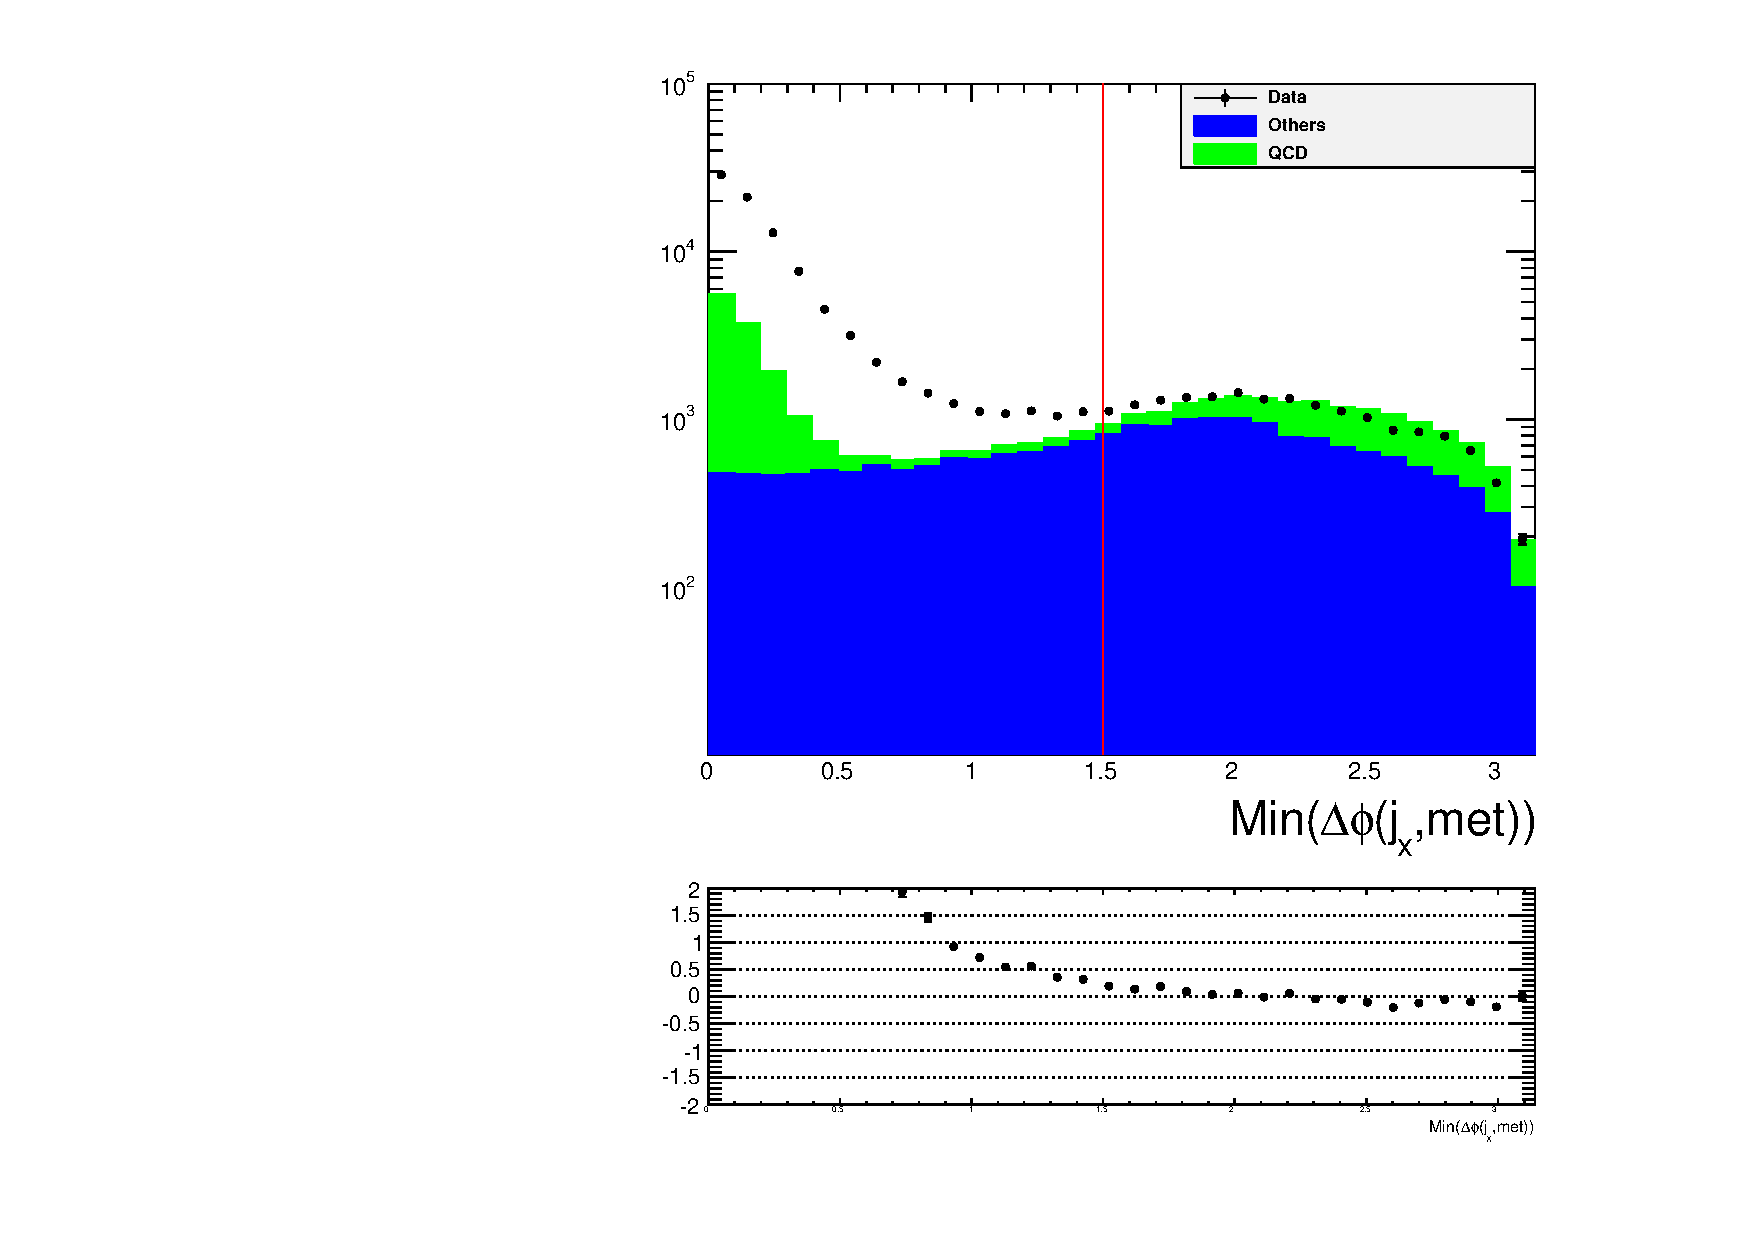
\includegraphics[width=\linewidth]{img/DEta3p6_MetSig3p0/jetmet_mindphi_LogY.pdf}

\end{block}

\column[t]{0.45\linewidth}
\begin{block}{Methodology}
 
\begin{itemize}
  \item We also know that one of the main reasons for fake MET is the miss measurement of the energy of one of the leading jets. 
  \item This typically results in MET being aligned with with the jets directions, which is reflected by the variable $Min(\Delta\phi(jet_{x},MET))$
  \item Again o repeat the procedure to used for MET significance 
  \item A good value is $Min(\Delta\phi(jet_{x},MET))=1.5$
  \item QCD normalised on $Min(\Delta\phi(jet_{x},MET))>1.5$ with $factor = \frac{n_{Data}-n_{\text{other bkg}}}{n_{QCD}}=1.50$ (compatible with NLO correction)
  \item Distribution matches well above cut.
\end{itemize}
 
\end{block}

\end{columns}

\end{frame}

% ###################################################
\begin{frame}{$Min(\Delta\phi(jet_{x},MET))$ cut - signal efficiency}
 
\begin{columns}
 
\column[t]{0.45\linewidth}
\begin{block}{Signal Eff. vs MET Significance}

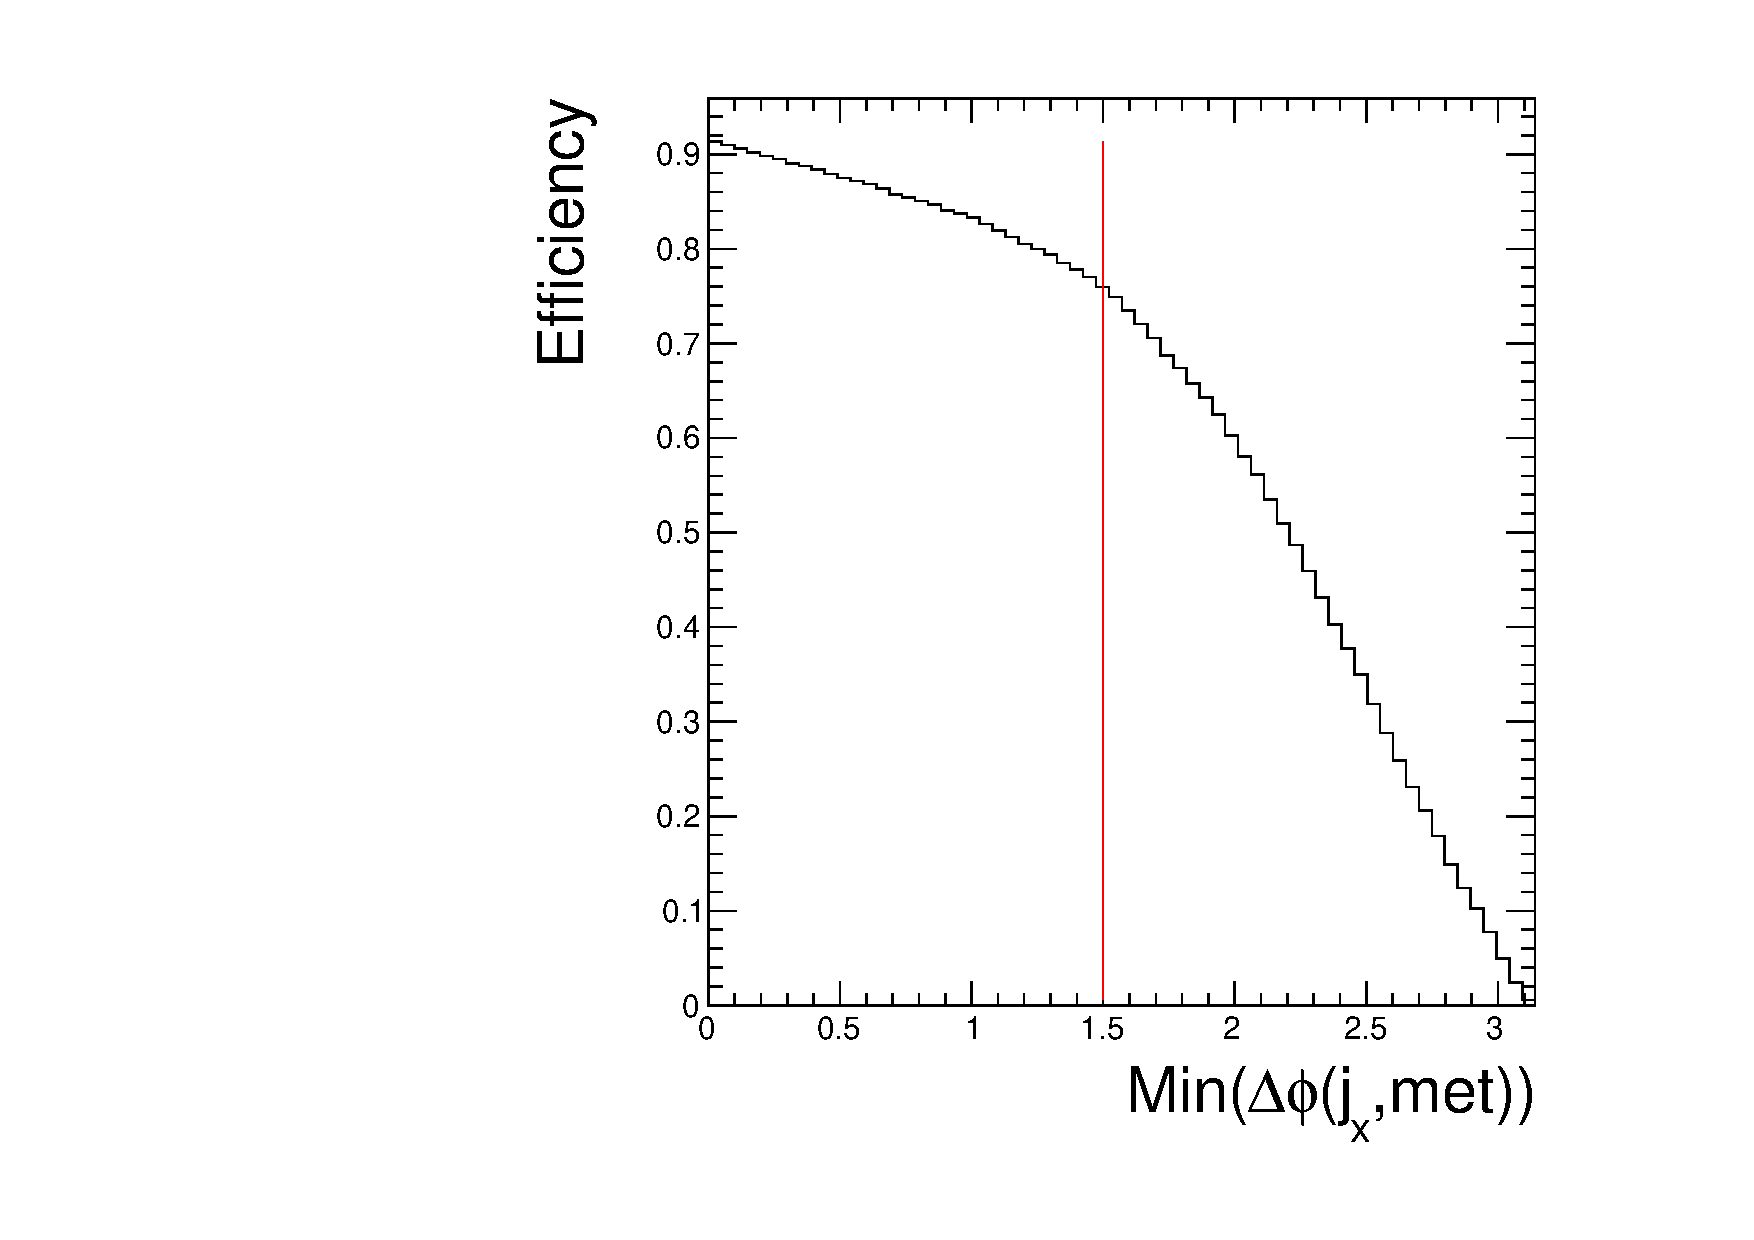
\includegraphics[width=\linewidth]{img/DEta3p6_MetSig3p0/DEta3p6_MetSig3p0_jetmet_mindphiEff.pdf} 

\end{block}

\column[t]{0.45\linewidth}
\begin{block}{}

Taking into account the previous cuts we can calculate:
\begin{itemize}
  \item Again for signal of $m_{Higgs}=125$ GeV and $BR(Inv)=100\%$ 
  \item Signal Efficiency $\Delta\phi$ (1.5) = $\sim0.76$
  \item Our signal is still at a comfortable level. 
\end{itemize}

\end{block}

\end{columns}

\end{frame}

% ###################################################
\begin{frame}{Looking at key variables}

At this point we already apparently reduced the fake MET content in data to a level that distributions match to a reasonable level. 

\begin{columns}
 
\column[t]{0.40\linewidth}
\begin{block}{Dijet Mass}
 
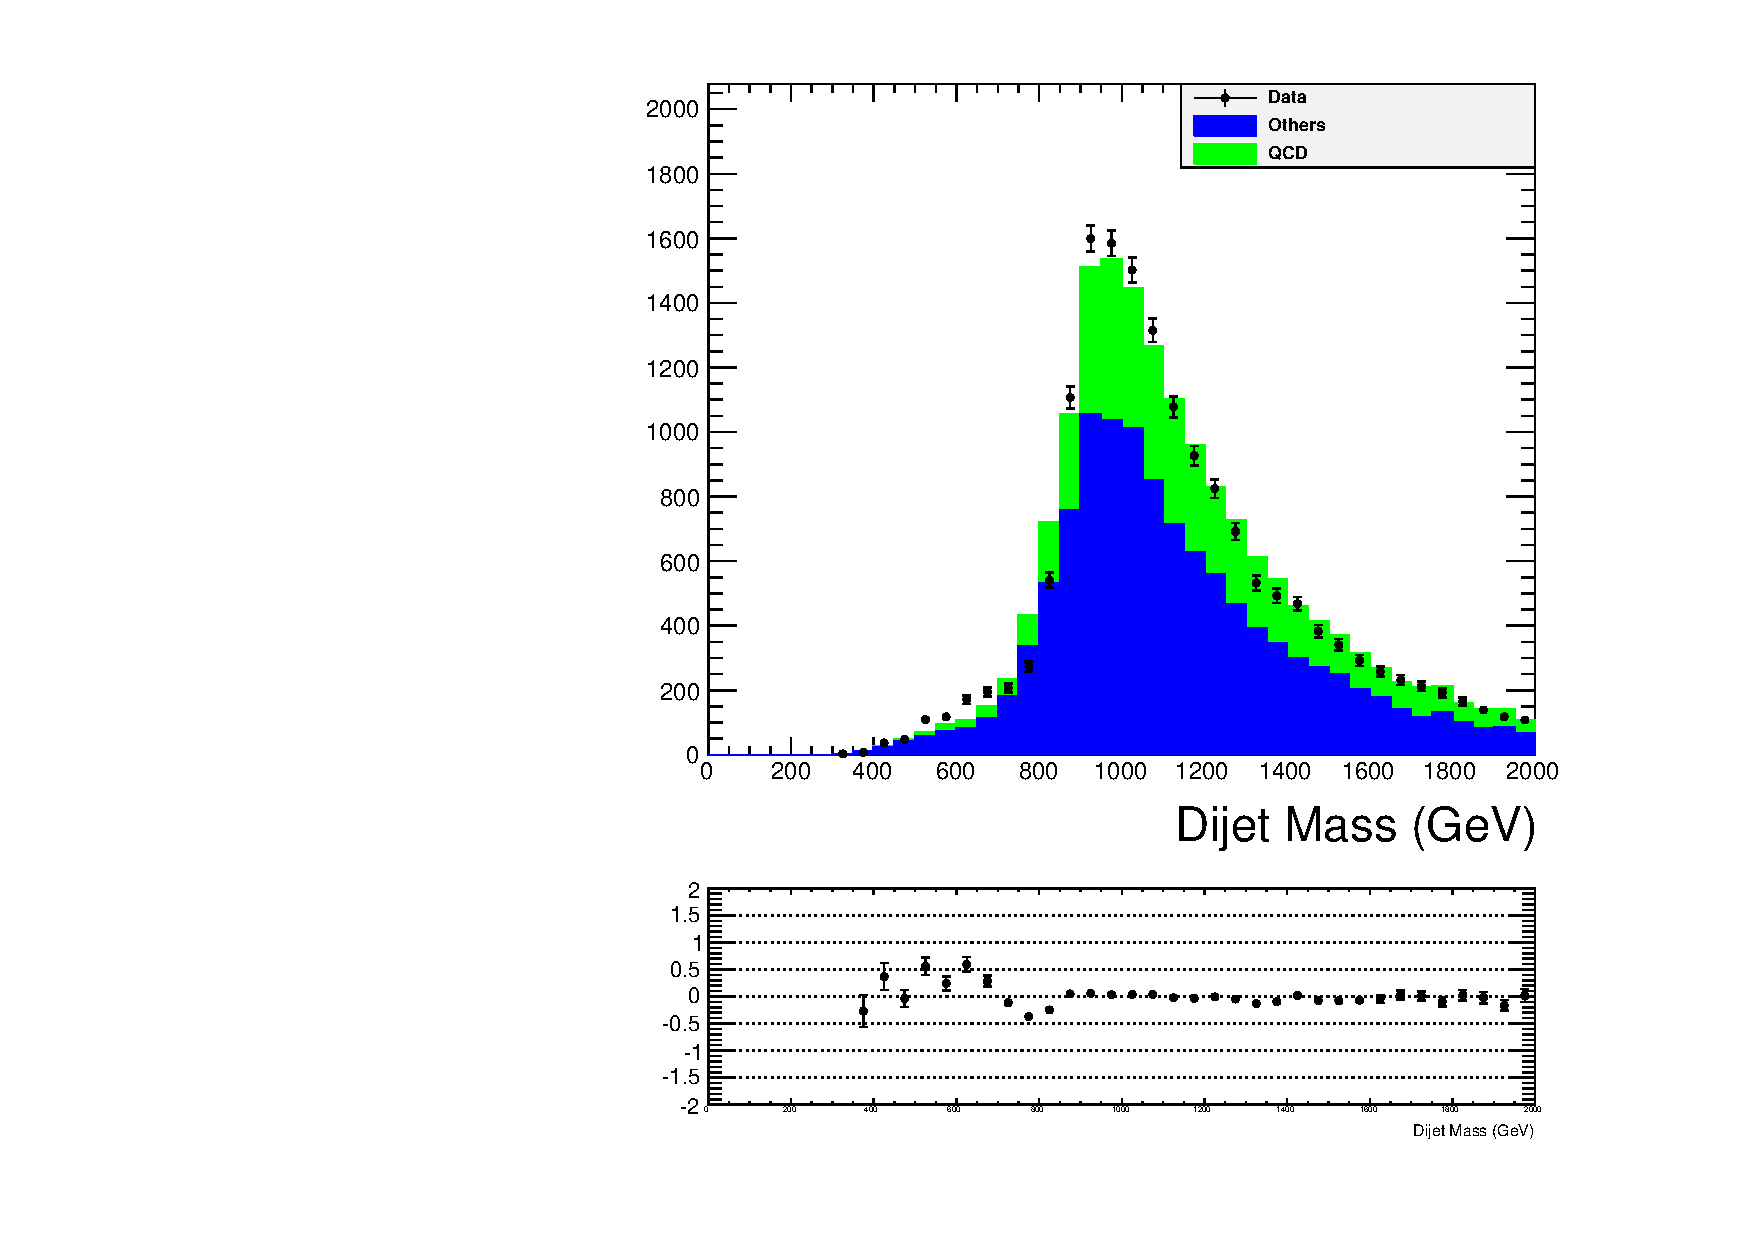
\includegraphics[width=\linewidth]{img/DEta3p6_MetSig3p0_MinDPhiJetsMet1p5/dijet_M.pdf}

\end{block}

\column[t]{0.40\linewidth}
\begin{block}{HT}

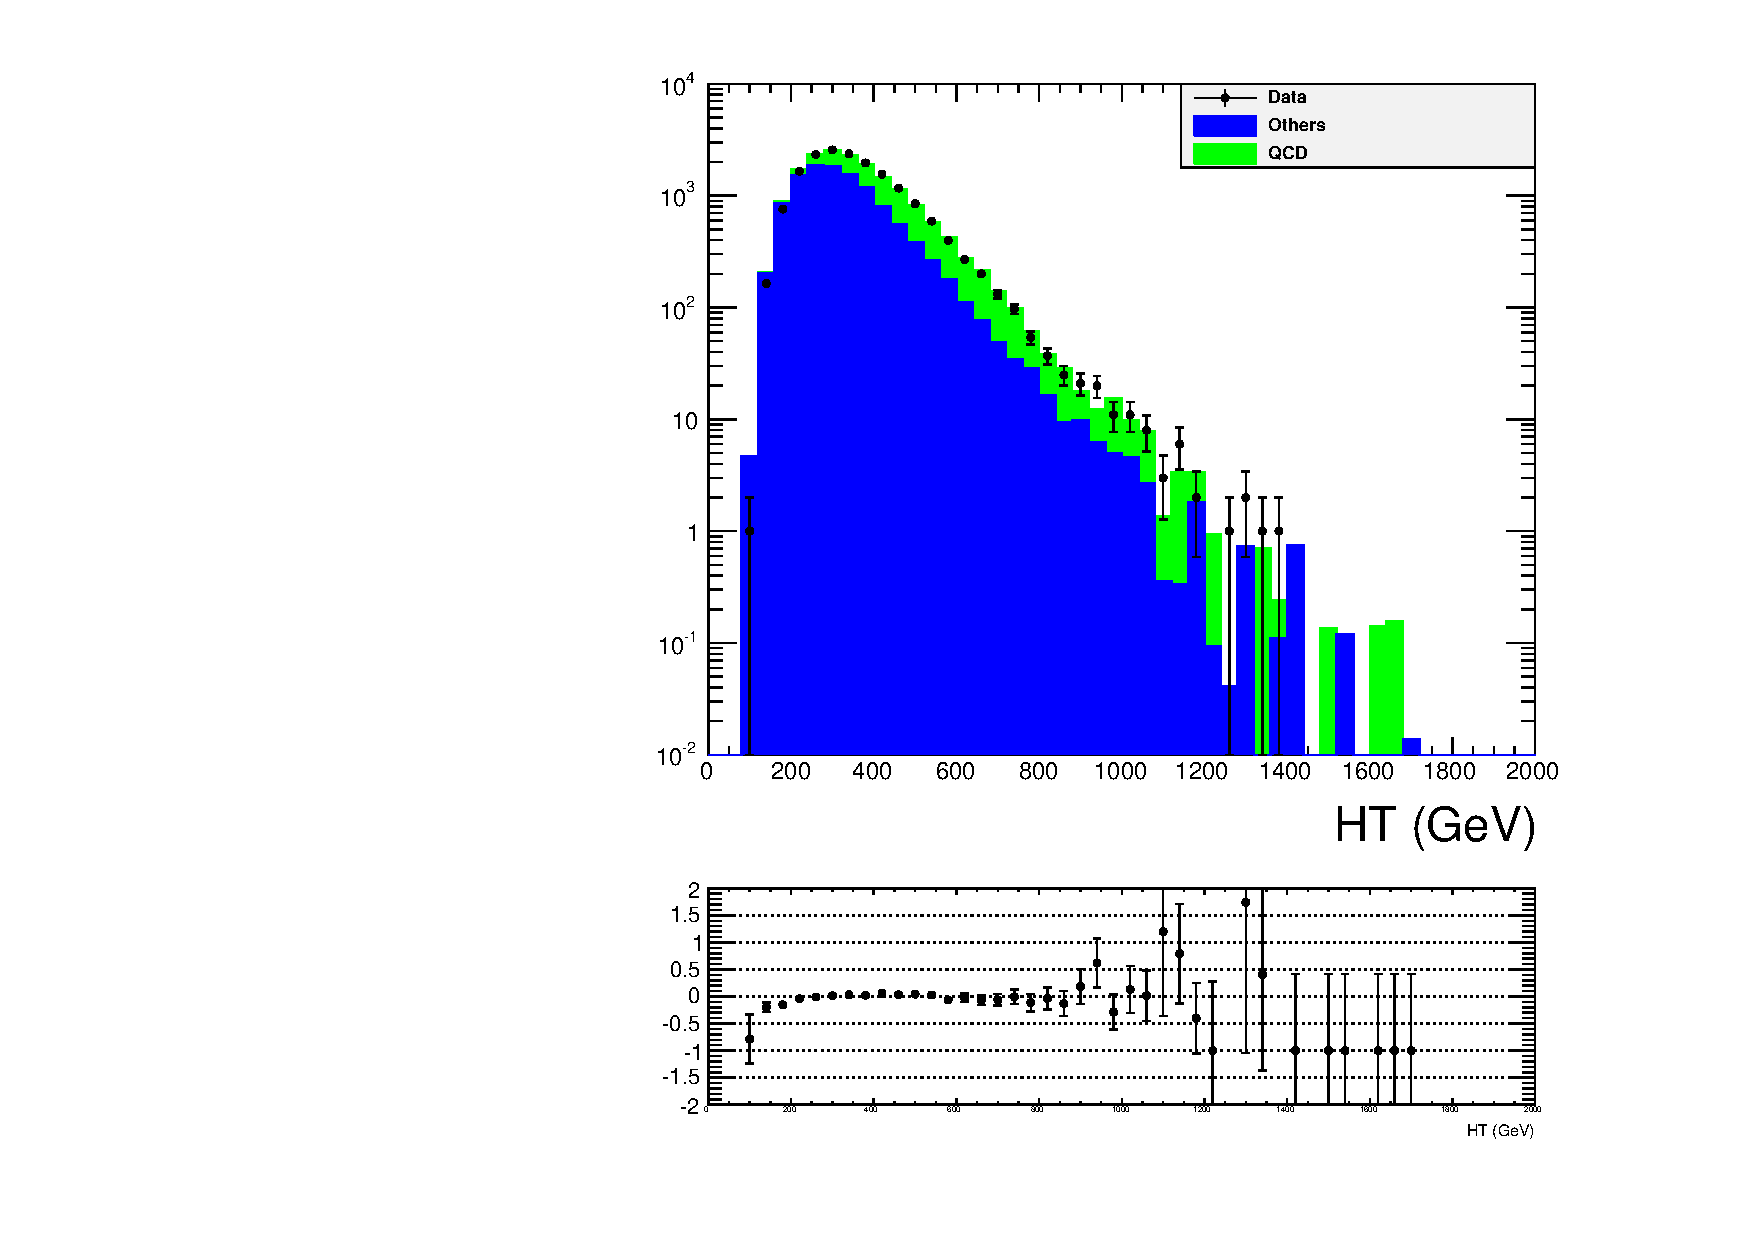
\includegraphics[width=\linewidth]{img/DEta3p6_MetSig3p0_MinDPhiJetsMet1p5/ht_LogY.pdf}
 
\end{block}

\end{columns}

\begin{block}

\tiny

For this point including this slide all distributions are normalised on the total number of expected yield passing all the cuts $factor = \frac{n_{Data}-n_{\text{other bkg}}}{n_{QCD}}$. This is not correct since
we can have signal on this regions, but is a good first approximation.

\end{block}

\end{frame}

% ###################################################
\begin{frame}{Dijet angles}

The dijet angles are reasonably described by the MC now and agreement if often of the order of $\sim10\%$ or better. But there is still room for improvement. 

\begin{columns}
 
\column[t]{0.45\linewidth}
\begin{block}{}
 
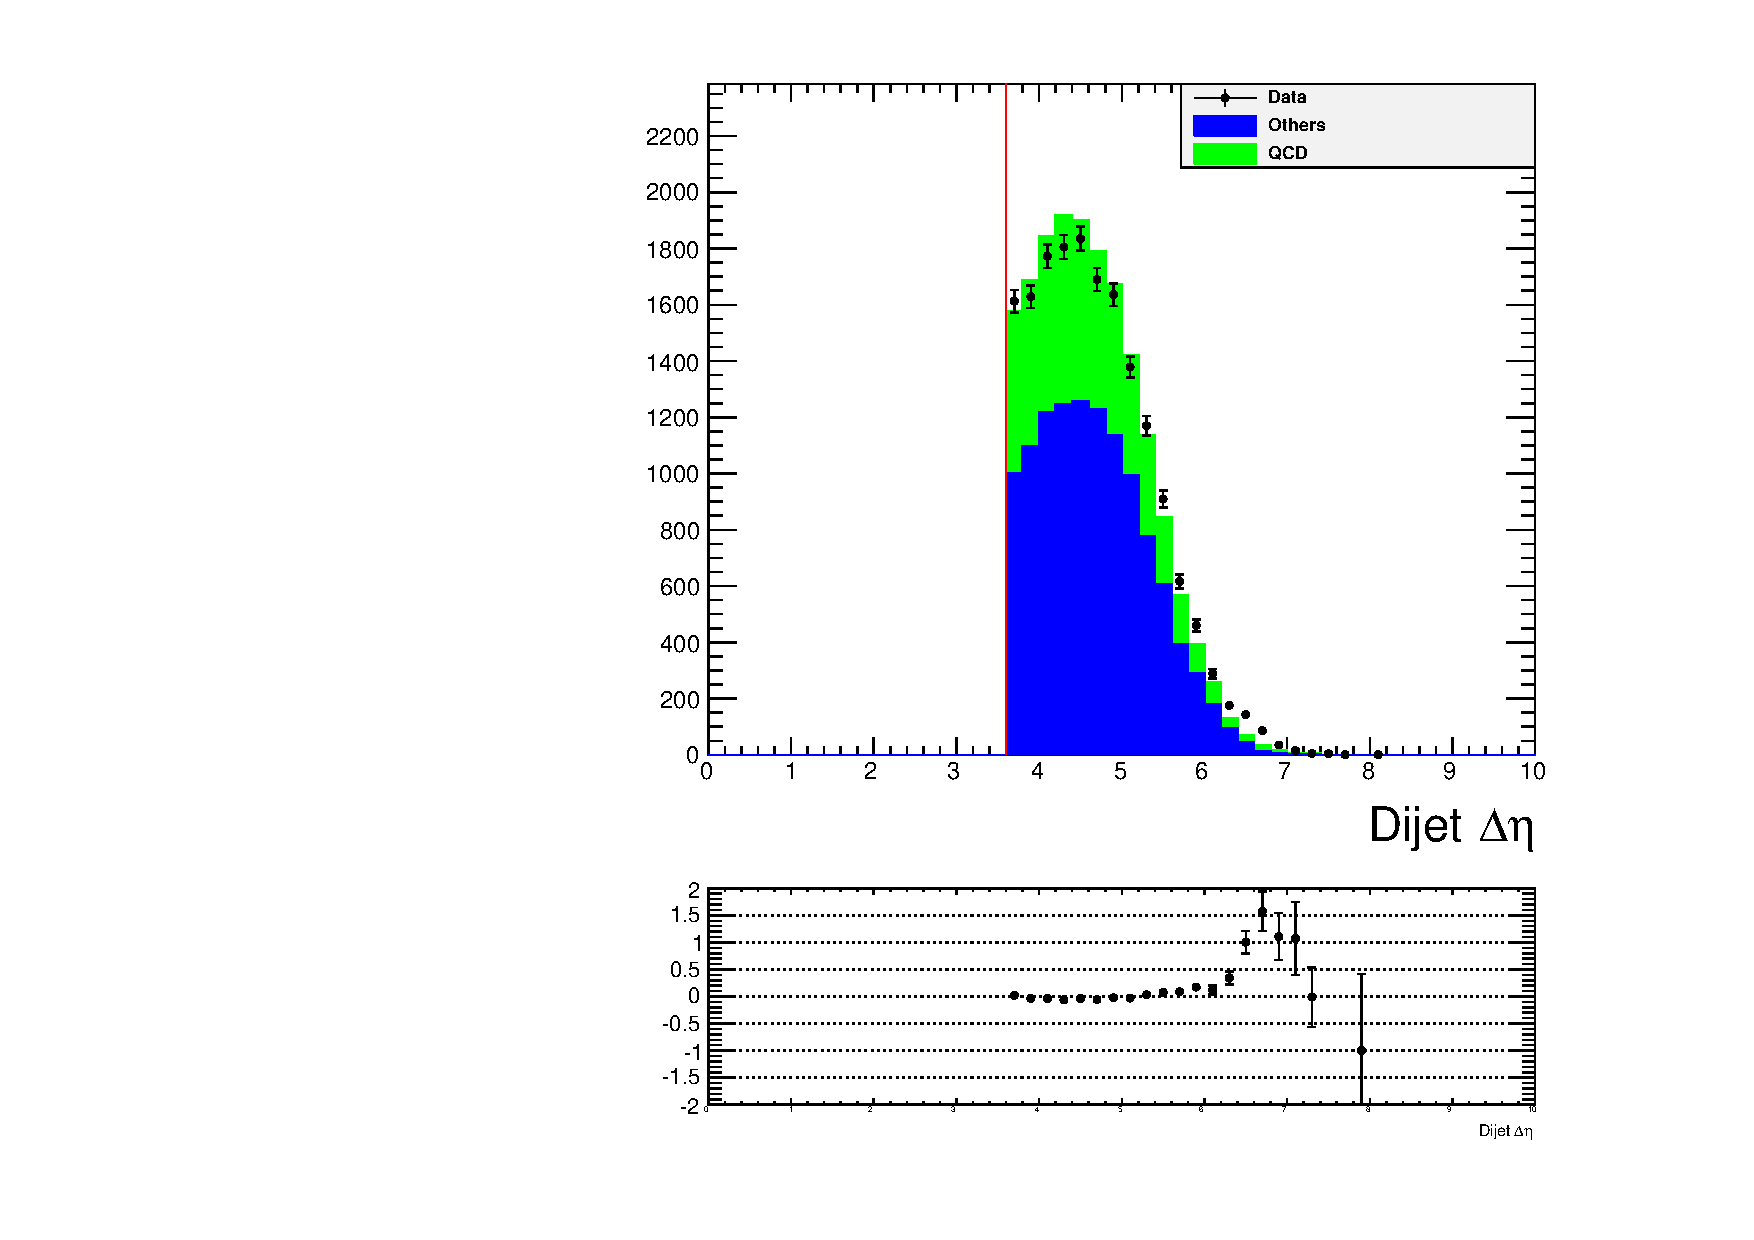
\includegraphics[width=\linewidth]{img/DEta3p6_MetSig3p0_MinDPhiJetsMet1p5/dijet_deta.pdf}

\end{block}

\column[t]{0.45\linewidth}
\begin{block}
 
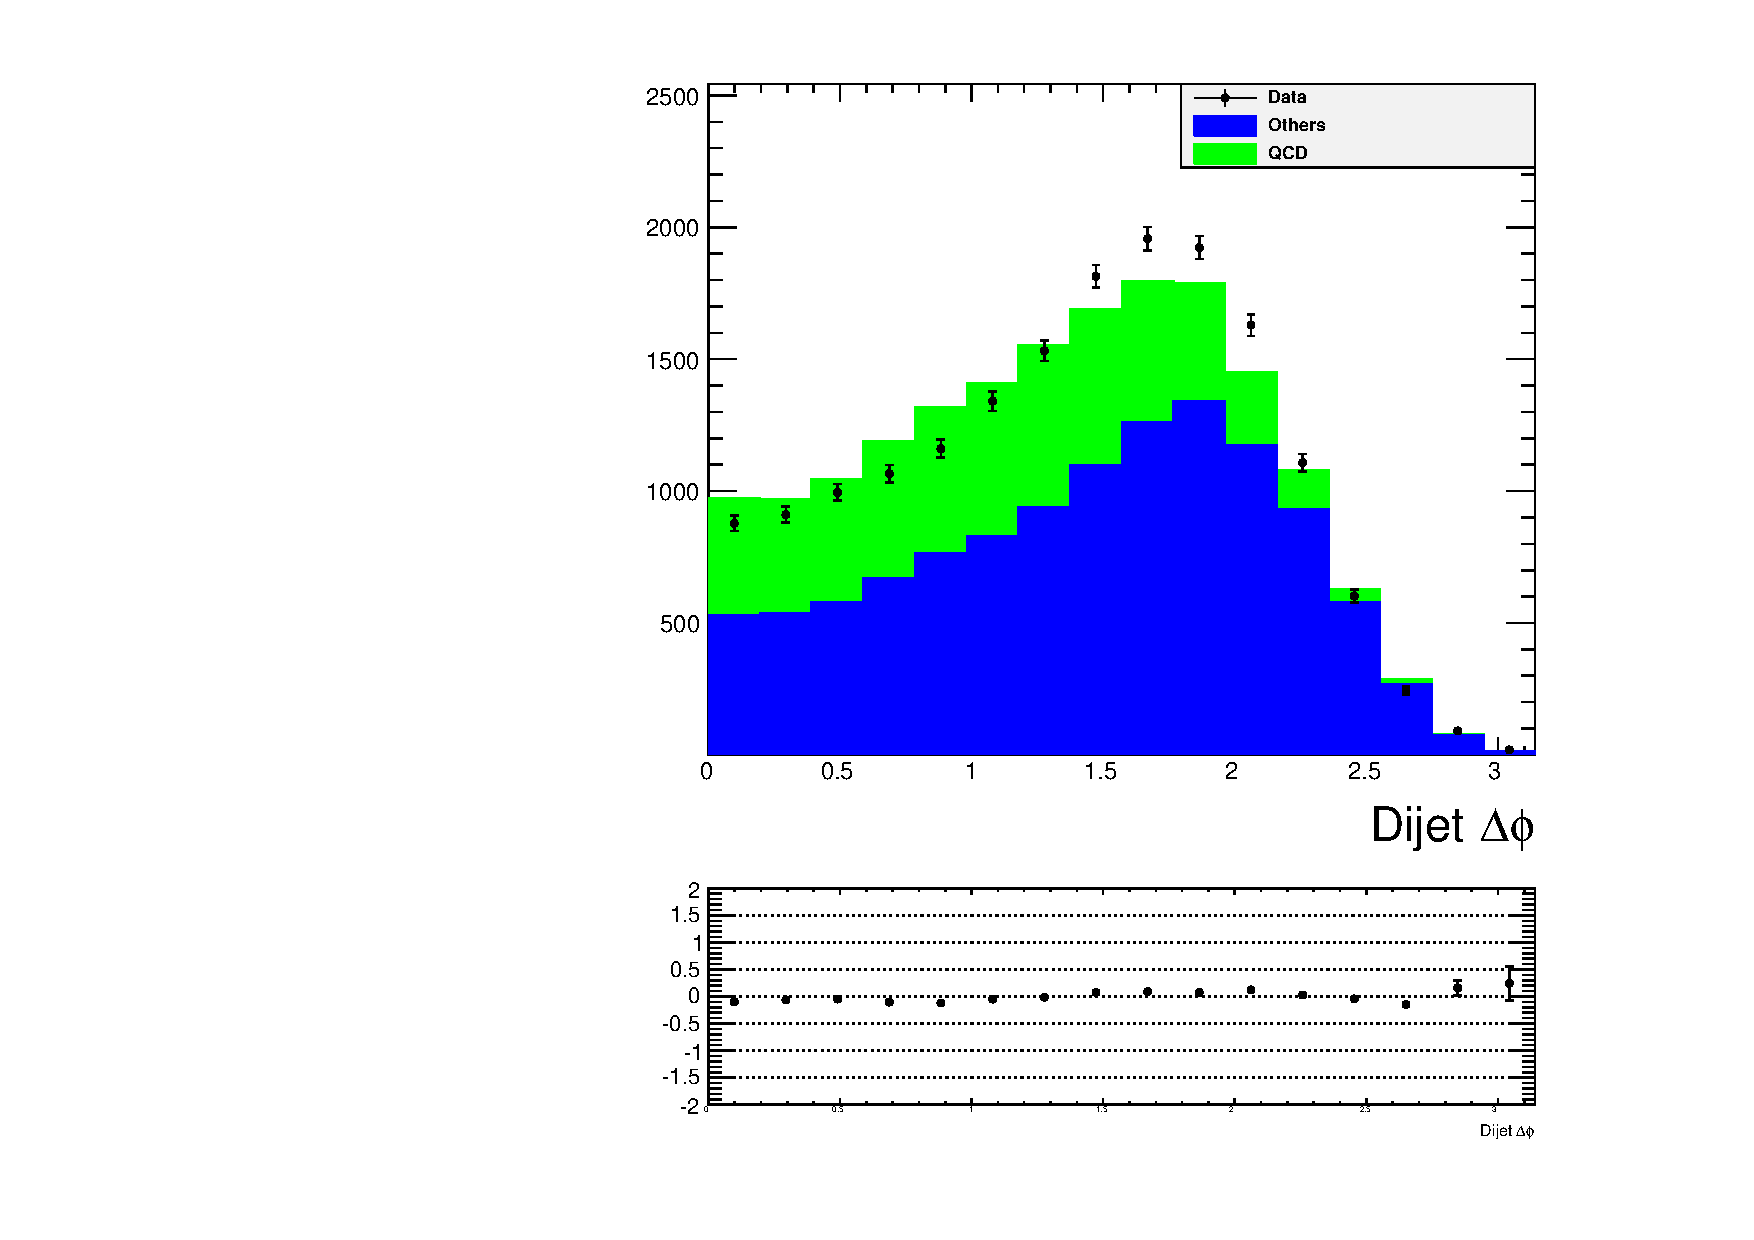
\includegraphics[width=\linewidth]{img/DEta3p6_MetSig3p0_MinDPhiJetsMet1p5/dijet_dphi.pdf}
 
\end{block}

\end{columns}

\end{frame}

% ###################################################
\begin{frame}{MET variables}

MET variables show some discrepancy but only at low values which are more likely to contain fake MET events. Further studies may allow to improve this.

\begin{columns}
 
\column[t]{0.45\linewidth}
\begin{block}{}
 
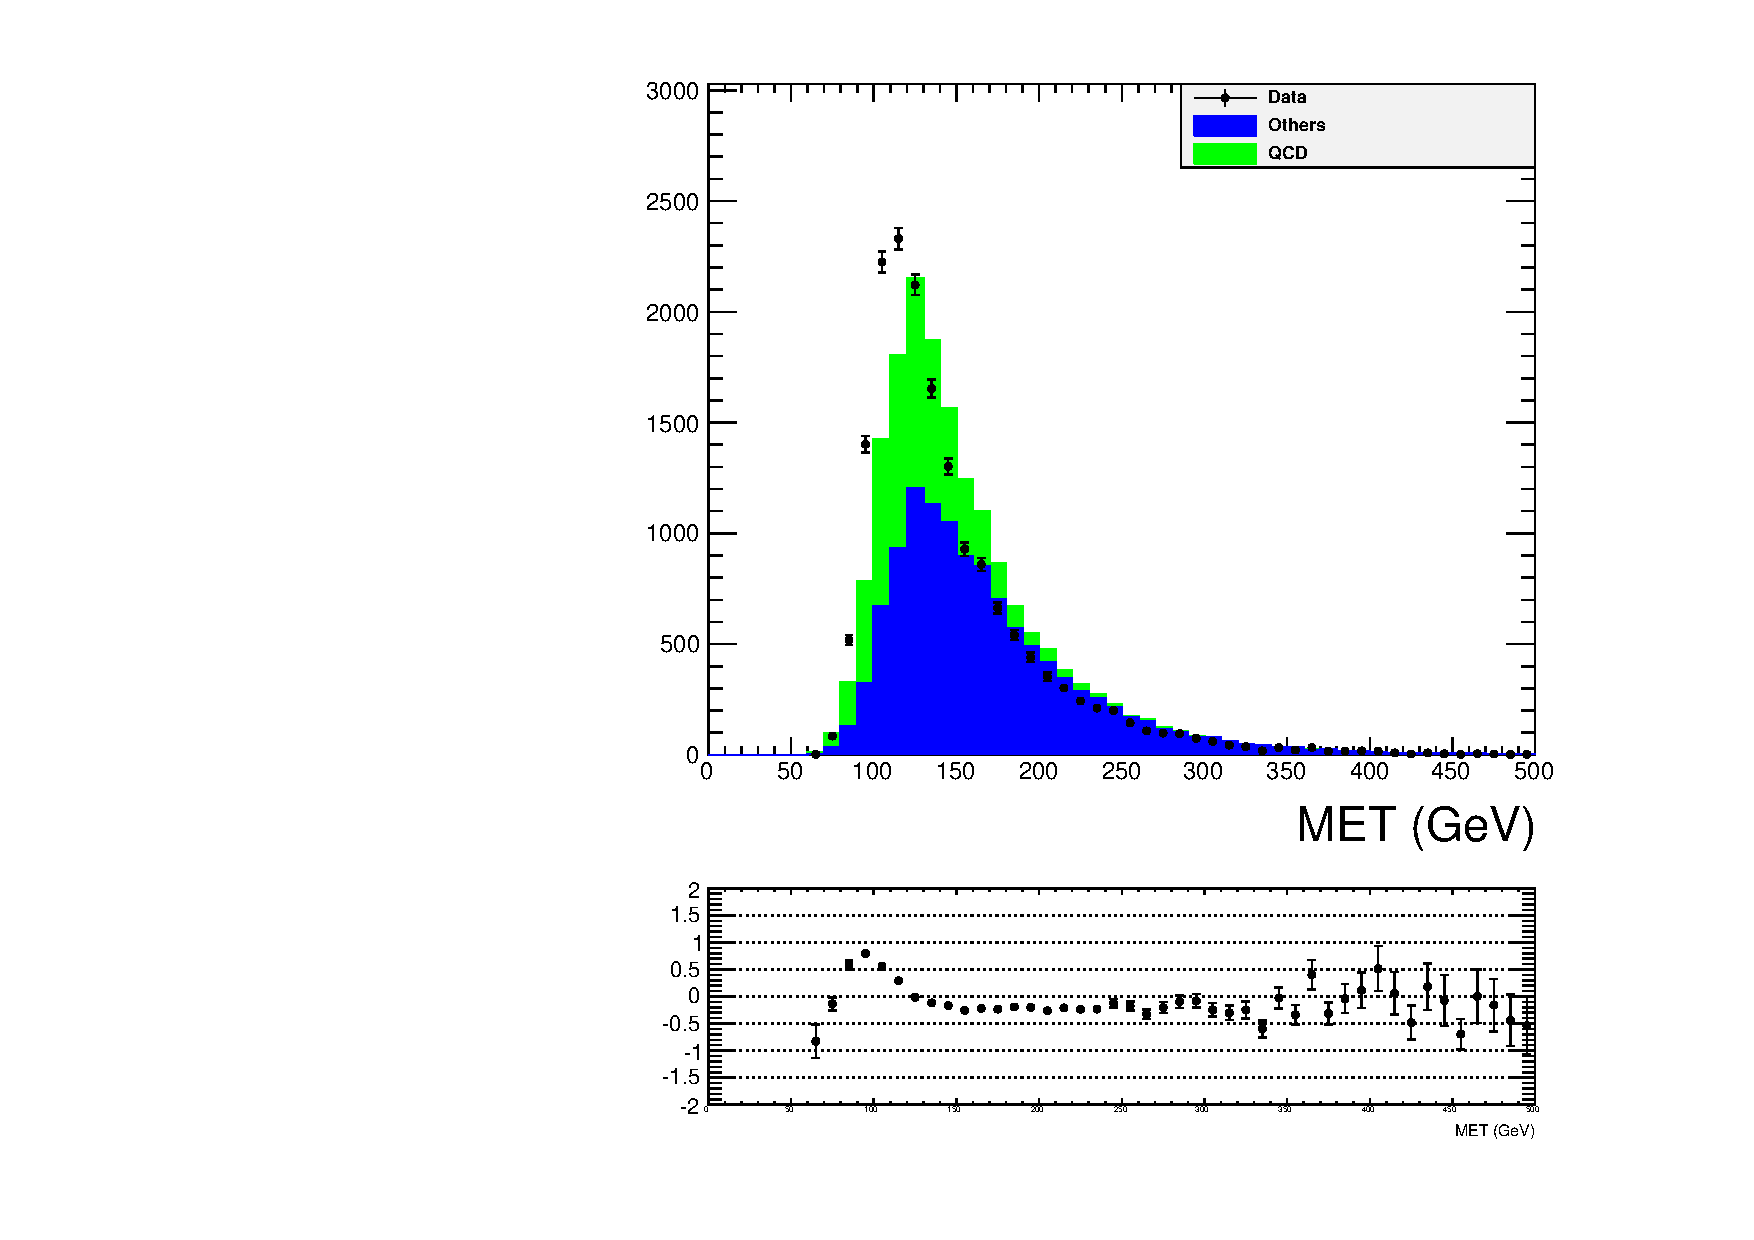
\includegraphics[width=\linewidth]{img/DEta3p6_MetSig3p0_MinDPhiJetsMet1p5/met.pdf}

\end{block}

\column[t]{0.45\linewidth}
\begin{block}
 
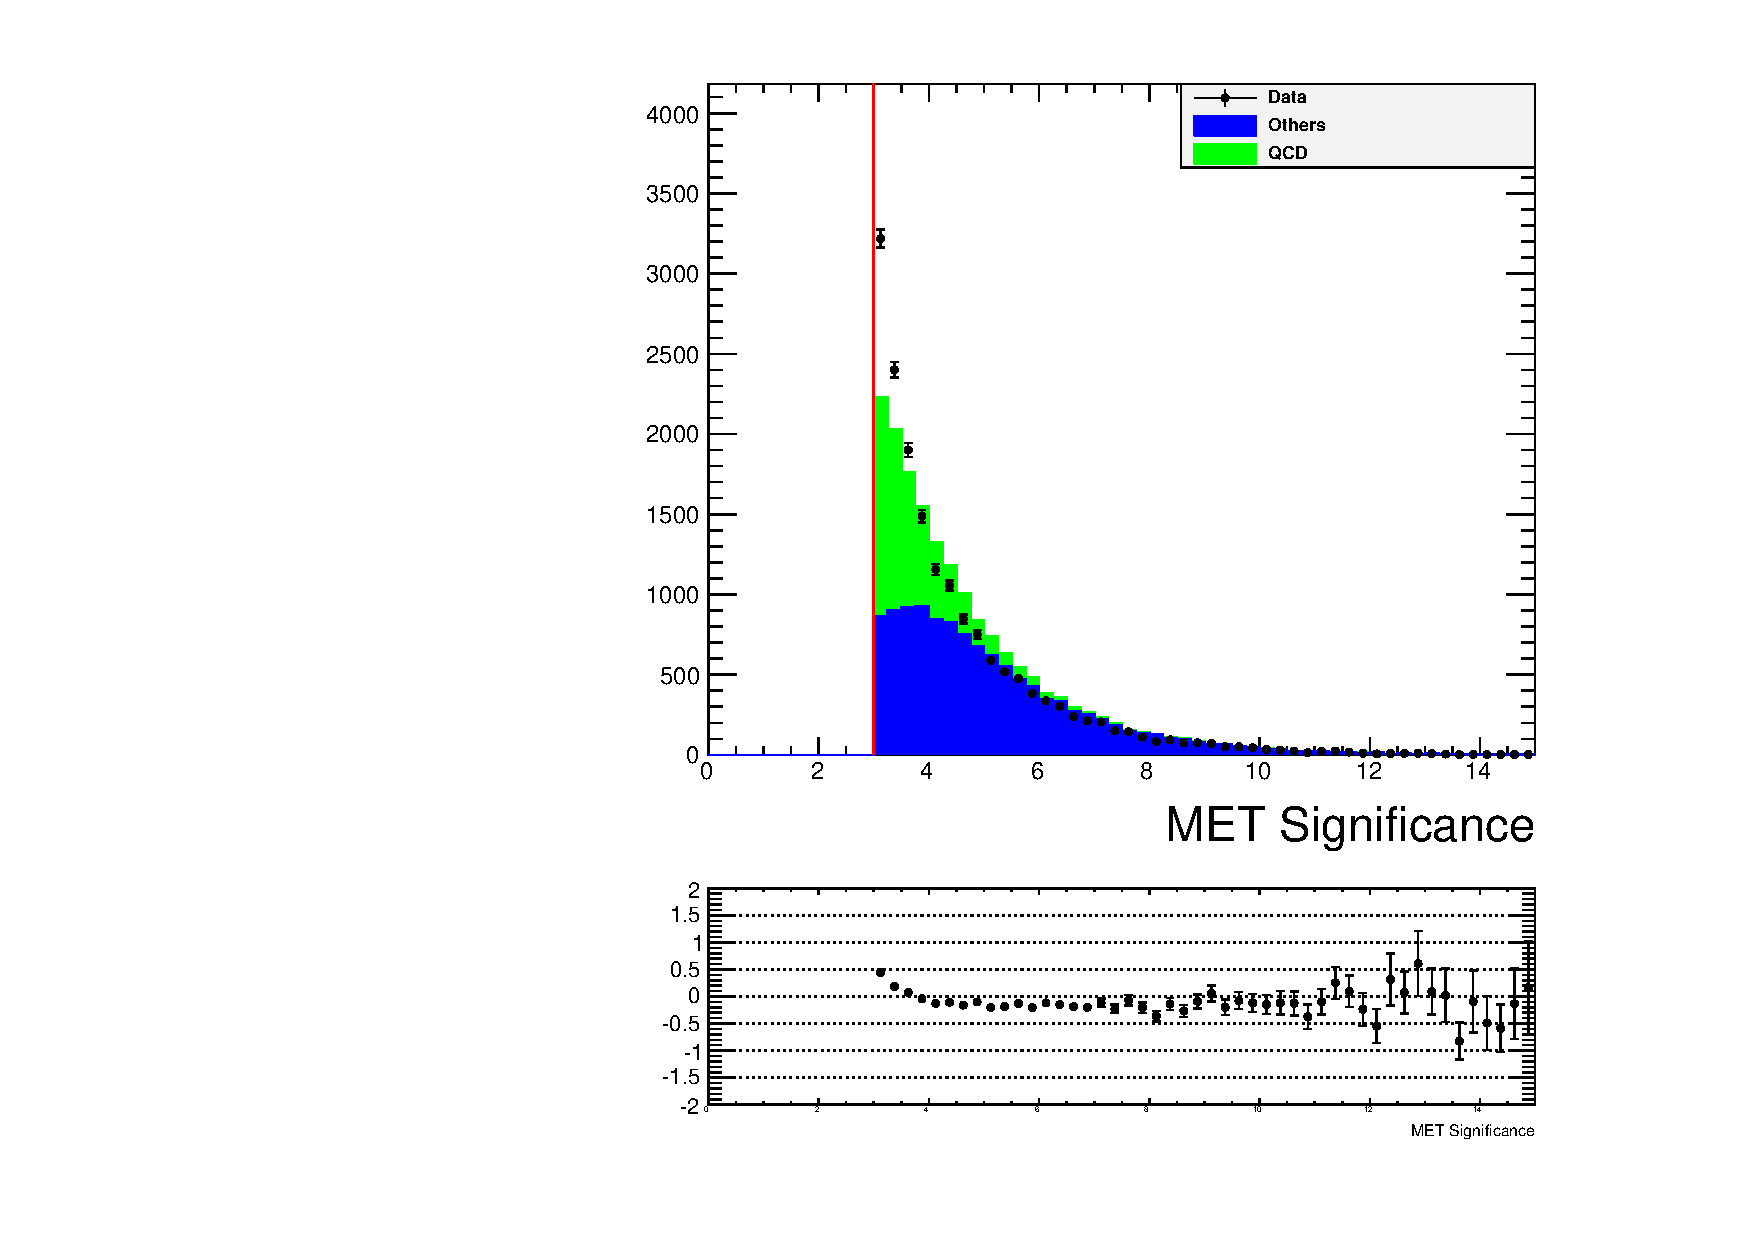
\includegraphics[width=\linewidth]{img/DEta3p6_MetSig3p0_MinDPhiJetsMet1p5/metSig.pdf}
 
\end{block}

\end{columns}

\end{frame}

% ###################################################
\begin{frame}{Effects now described}

\begin{columns}
 
\column[t]{0.45\linewidth}
\begin{block}{}
 
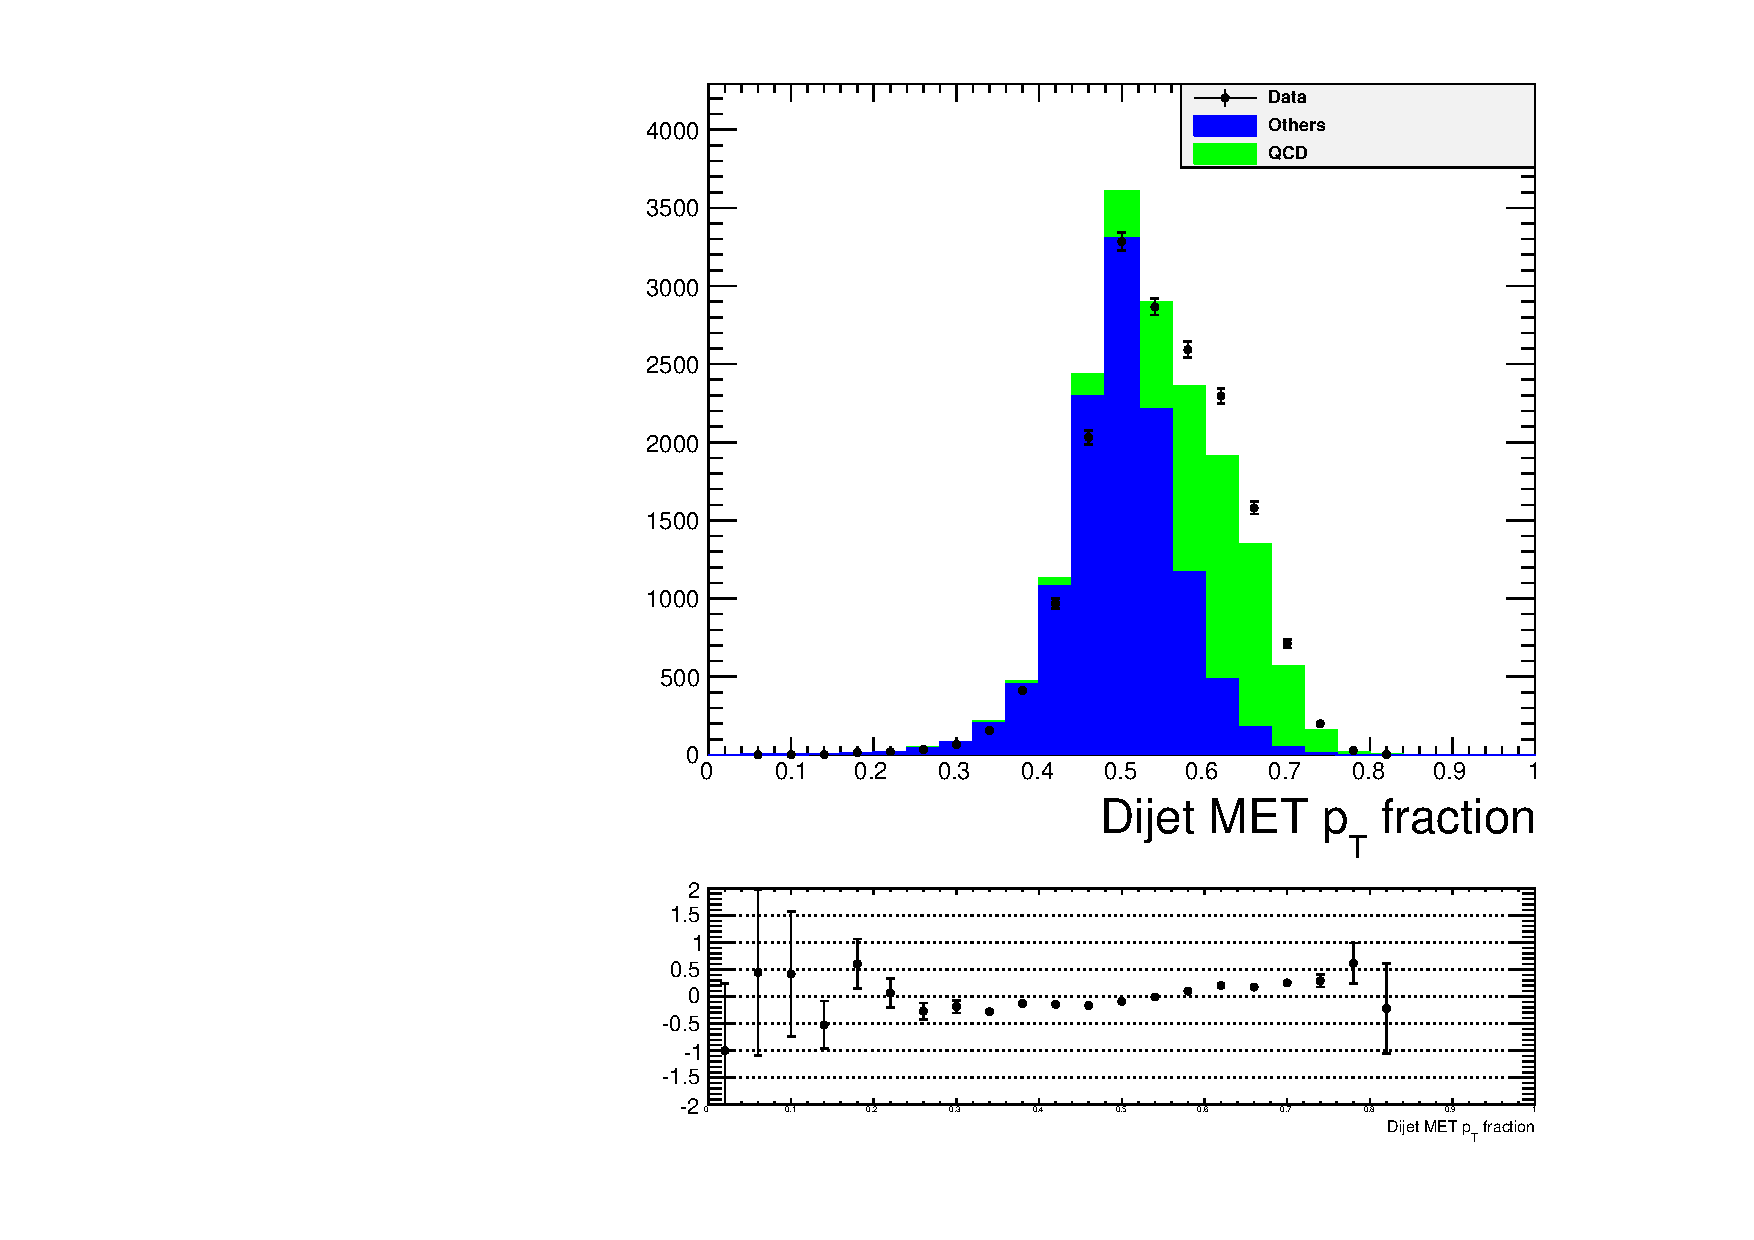
\includegraphics[width=\linewidth]{img/DEta3p6_MetSig3p0_MinDPhiJetsMet1p5/dijetmet_ptfraction.pdf}

\end{block}

\column[t]{0.45\linewidth}
\begin{block}

\begin{itemize}
  \item Now for the first time we can actually model the excess on data while compared with other backgrounds observed at high values of Dijet-MET $p_{\perp}$ fraction.
  \item This excess as expected comes from QCD and this variable is therefore discriminate against that type of backgrounds. 
\end{itemize}

\end{block}

\end{columns}

\end{frame}


% ###################################################
\begin{frame}{Analysis Strategy}

\begin{block}{QCD VBF samples}
 
Now that we found a pre-selection that is a reasonable working point where our MC samples can describe data. We can use it as a baseline to the rest of the analysis.

\end{block}

\begin{block}{BDT approach}
 
\begin{itemize}
 \item We can drop the QCD exclusion BDT
 \item We can make an all background against signal BDT 
 \begin{itemize}
   \item Trained starting from this or a similar pre-selection
   \item Use as a basis for training the QCD VBF sample
   \item This would be a single BDT approach
  \end{itemize}
\end{itemize}
 
Data driven methods still necessary to full understand all steps including pre-selection. 
 
\end{block}
 
\end{frame}

{
\setbeamercolor{background canvas}{bg=}
\includepdf[pages=9]{hinv_magnan_140506.pdf}
}

{
\setbeamercolor{background canvas}{bg=}
\includepdf[pages=10]{hinv_magnan_140506.pdf}
}

{
\setbeamercolor{background canvas}{bg=}
\includepdf[pages=12]{hinv_magnan_140506.pdf}
}

% {
% \setbeamercolor{background canvas}{bg=}
% \includepdf[pages=13]{hinv_magnan_140506.pdf}
% }

{
\setbeamercolor{background canvas}{bg=}
\includepdf[pages=14]{hinv_magnan_140506.pdf}
}

\begin{frame}{Rough limits calculation \hfill(P. Dunne)}
 
\begin{block}{Assumptions:}
 
\begin{itemize}
  \item Same background expectation from cut based
  \item Increasse in signal yield of 20 events (~5\%)
  \item Same systematics
\end{itemize}

\end{block}
 
The limit on BR(Inv) goes from 65\% to 55\% so a gain of around 10\%.
 
\end{frame}

% ###################################################
% \begin{frame}{Further ideas for the analysis}
%  
% If one of the main signal losses now can become combinatorics we can select an orthogonal data region to out signal based on selecting instead of $1^{st}$ and $2^{nd}$ leading jets.
%  
% \begin{block}{Method}
%  
% \begin{itemize}
%   \item Select $1^{st}$ and $3^{rd}$ or $2^{nd}$ and $3^{rd}$ leading jets.
%   \item Ignoring the $2^{nd}/1^{st}$ (assume it is miss measured) 
%   \item Proceed with normal selection
% \end{itemize}
% 
% \end{block}
%  
% \end{frame}

% ###################################################
\begin{frame}{Summary and next steps}
 
\begin{block}{Summary:}
 
\begin{itemize}
  \item A good working point for a pre-selection was found
  \item Reasonable agreement of key variables and data is observed
  \item Normalisation needs to be revisited to avoid signal contamination
  \item New possible structure for the analysis presented based on this findings 
  \item With similar working point to current in cut based we can improvement of 10\% in the limit
\end{itemize}

\end{block}

\begin{block}{Next Steps:}
 
\begin{itemize}
  \item Optimise pre-selection
  \item Optimise and study BDT approach
  \item Calculate yield/limit gains with parked data 
\end{itemize}
 
\end{block}

\end{frame}


% ###################################################
\appendix
% ###################################################
\begin{frame}
 
\begin{block}

\begin{center}Backup Slides\end{center}

\end{block}

\end{frame}

{
\setbeamercolor{background canvas}{bg=}
\includepdf[pages=11]{hinv_magnan_140506.pdf}
}

\end{document}